\documentclass[11pt]{article}
\usepackage{geometry}
\geometry{
 a4paper,
 total={210mm,297mm},
 left=20mm,
 right=20mm,
 top=20mm,
 bottom=20mm,
 }
 
\usepackage[english]{babel}
\usepackage[utf8x]{inputenc}
\usepackage{amsmath}
\usepackage{graphicx}
\usepackage[table,xcdraw]{xcolor}
\usepackage[colorinlistoftodos]{todonotes}
\usepackage{multicol}
\usepackage{ragged2e}
\usepackage{tocloft}
\usepackage{titlesec}
\usepackage{natbib}
\usepackage[parfill]{parskip}
\usepackage{amssymb}
\usepackage{textcomp}
\usepackage{float}
\floatstyle{plain}
\usepackage{color}
\usepackage{epstopdf}
\usepackage{hyperref}
\usepackage{comment}
\hypersetup{
    colorlinks=true,
    linkcolor=blue,
    filecolor=magenta,      
    urlcolor=cyan,
    citecolor=blue
}
\urlstyle{same}
\usepackage{fancyhdr}
\usepackage{lipsum}
\usepackage{subscript}
\usepackage{siunitx}
\usepackage[hypcap]{caption}
\usepackage{capt-of}
\usepackage{wasysym}
\usepackage{wrapfig}
\usepackage{enumitem}
\usepackage{pdflscape}
\usepackage{pdfpages}
\usepackage{csquotes}

%making the bloody title 
\makeatletter
\renewcommand{\maketitle}{\bgroup\setlength{\parindent}{0pt}
\begin{flushleft}
  \textbf{\@title} %the empty line is impt

  \@author
\end{flushleft}\egroup
}
\makeatother

%random things needed
%\renewcommand{\cftsecleader}{\cftdotfill{\cftdotsep}} %let the content table have dots to number
\linespread{1.5}  %making one and a half spacing-sh one and half is actually 1.3
\frenchspacing
%\titlespacing\subsection{0pt}{12pt plus 4pt minus 2pt}{0pt plus 2pt minus 2pt} 
\titlespacing\subsubsection{0pt}{12pt plus 4pt minus 2pt}{0pt plus 2pt minus 2pt} %less spacing between subsubsections
\pagestyle{fancy}
% Set the right side of the footer to be the page number
\fancyhf{} % sets both header and footer to nothing
\renewcommand{\headrulewidth}{0pt}
\fancyfoot[R]{\thepage}
\fancypagestyle{plain}{%
    \renewcommand{\headrulewidth}{0pt}%
    \fancyhf{}%
    \fancyfoot[R]{\thepage}%
}
\setlength{\parskip}{0pt}

%insert title
\title{\textbf{\huge{The Evolution of Echolocation in Bats }}}
\date{} 
\author{%
\large{ Jia Le, Lim {  } CID: 00865029 } \\
\textnormal
{\textit{Department of Biology, Imperial College London, South Kensington Campus, London, U.K.}} \\
Submitted: 20 Jan 2017
}

\begin{document}
\maketitle
%space after title
\bigskip

\tableofcontents

\section{Phylogeny of Bats}

Bats comprise of around one-fifth of all mammalian species and are the only mammals with self-powered flight and the ability to use laryngeal echolocation~\citep{Teeling2009}. Moreover, bats are found all around the world and are crucial pollinators and insect predators of the ecosystem. Despite their importance, the evolutionary history of bats remained unclear until recently due to insufficient fossil records and numerous conflicting phylogenetic hypotheses~\citep{Teeling2005}. In fact, Charles Darwin once suggested in the \textit{Origin of Species} that the sudden evolution of bats with flight and echolocation capabilities from insectivorous terrestrial mammals was too unparsimonious for it to have occurred via natural selection~\citep{Darwin1859a}.
\\
\\
Nonetheless, molecular dating indicates that crown-group bats first made their appearance around 64 million years ago when they diverged from other groups within the Laurasiatheria. Subsequently, crown-group bats diversified in a short time frame during the early Eocene~\citep{Teeling2009}. Traditional morphological data divides the monoclade of bats into two suborders, the Megachiroptera and the Microchiroptera. Megachiroptera consists of the Old World fruit bats, which have specialised nocturnal vision, while Microchiroptera contains the microbats, which uses laryngeal echolocation~\citep{Jones2006}. 
\\
\\
Although recent molecular data support the chiropteran monophyly, the analysis of 13.7 kilobases of nuclear sequence data also revealed the paraphyly of its two suborders. It is now generally accepted that all megachiropterans, along with some microchiropteran species group together under a new clade named the Yinpterochiroptera while the rest of the microchiropterans are placed together under the suborder Yangochiroptera~\citep{Teeling2005}. This raises the question of whether laryngeal echolocation evolved once and was subsequently lost in the Old World fruit bats or if it evolved twice independently~\citep{Teeling2009}.
%%%%%

\section{Echolocation}

Laryngeal echolocation is a complex trait that is influenced by multiple genes that are involved in many physiological pathways. To echolocate, bats must evolve the ability to generate high-frequency calls using their larynx, hear and receive returning echoes as well as be able to understand such returning echoes~\citep{Teeling2009}. 
%%%%
\\
\\
Specialised hearing that is both sensitive and selective to high-frequency sound is hence crucial in bats. A major auditory system of the inner ear, the cochlea, is well-developed in bats and the cochleae of echolocating bats and whales show convergent anatomical characteristics, such as the presence of shorter and stiffer outer hair cells (OHCs) in comparison with other mammals~\citep{Liu2010}. OHCs, located in the organ of Corti in the cochlea, transform incoming sound waves into nerve impulses~\citep{Robles}. Thus, it is unsurprising that the expressions of several echolocation genes have been found in OHCs of bats~\citep{Davies2012, Li2008a, Liu2012}.
\\
\\
Moreover, echolocating bats have an adapted nervous system involved in transmitting and processing auditory signals. Their central nervous systems display similar structural characteristics as those of most other mammals. However, some pathways, such as the auditory-motor pathways, exhibit hypertrophy and are sometimes arranged differently from those in non-echolocating species~\citep{Covey2005}. Additionally, echolocating bats, when compared to non-echolocating mammals, exhibit expanded regions of their cerebellum~\citep{Paulin1993a}. A few echolocation genes, which are expressed in neurons and parts of the brains, have also been recently identified~\citep{Davies2012, Li2007a}.
\\
\\
By comparing genes involved in echolocation among different bat species, we will be able to determine if both echolocating lineages use the same mechanisms for echolocation and if there exists any supporting evidence of the loss of such mechanisms in non-echolocating lineages. Similar proteins found in all bat species will hence support the hypothesis that echolocation evolved only once in bats. Otherwise, convergent evolution of echolocation in the two lineages of bats would indicate that echolocation is a non-homologous trait~\citep{Teeling2009}(\autoref{fig:phylogeny}).
\smallskip
\begin{figure}[H]
  \centering
    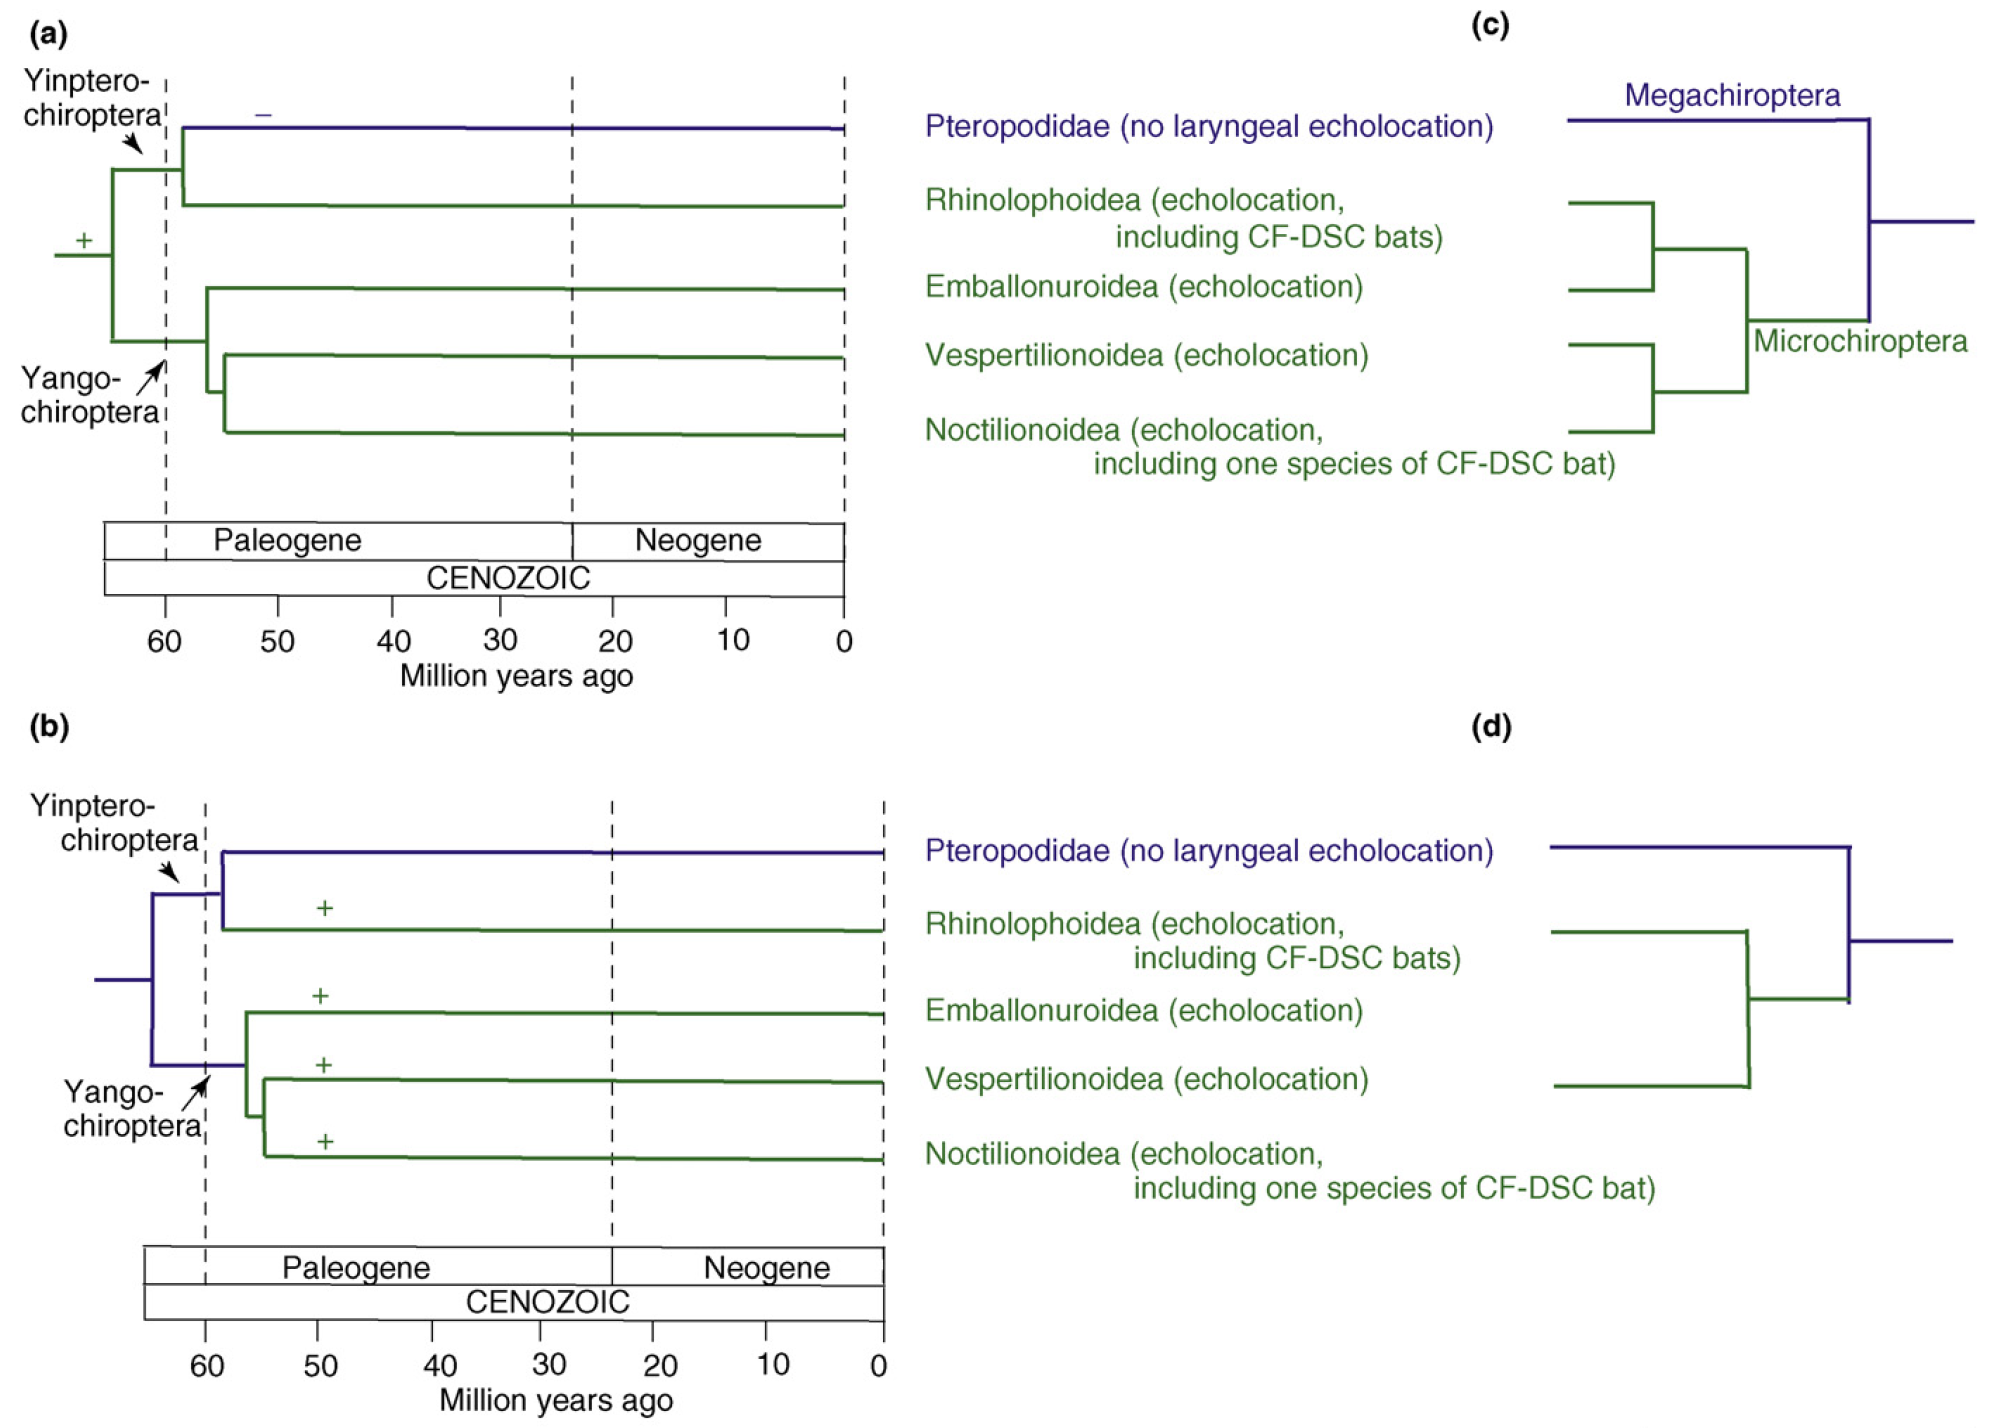
\includegraphics[width=\textwidth]{phylogeny.png}
  \captionof{figure}{\textbf{The two hypotheses of the evolution of echolocation in bats.} \footnotesize  \textbf{(a, b)} The currently widely accepted phylogenetic tree of bats, drawn with respect to estimated divergence times. Gain of echolocation is suggested at points with green `$+$'  while loss of echolocation is suggested at points with purple `$-$'. (a) Single point of evolution of echolocation in crown-group bats, followed by subsequent loss of echolocation in pteropodids, Old World fruit bats. (b) Convergent and independent evolution of echolocation in the different echolocating lineages. \textbf{(c, d)} The traditional phylogeny of bats that exhibits the monophyly of echolocators, as shown by several gene trees of echolocation genes. (Taken from~\cite*{Teeling2009}).}
  \label{fig:phylogeny}
\end{figure}


\subsection{Molecular Cues in the Cochlea}

\subsubsection{Prestin}
The first and most well-known example is prestin. Prestin belongs to the SLC26 superfamily of anion transporters and is a membrane motor protein present on OHCs~\citep{Zheng2000}. It is encoded by \textit{Prestin} and contains intracellular amino and carboxyl termini with 10-12 transmembrane domains~\citep{Li2008a}. Targeted deletion of \textit{Prestin} results in loss of cochlea sensitivity to sound in mice~\citep{Liberman2002}. Similarly, mutations in \textit{Prestin} are responsible for recessive non-syndromic deafness in humans, indicating its significance in auditory processing~\citep{Liu2003}. In echolocating bats, the non-synonymous substitution rate of \textit{Prestin} has been estimated to be higher than its synonymous substution rate. This indicates the presence of positive selection for prestin and highlights the importance of this protein in echolocation~\citep{Li2008a}. 
\\
\\
DNA sequences of \textit{Prestin} in 12 echolocating and non-echolocating bat species were sequenced and thereafter used to generate a phylogenetic tree. The resulting gene tree grouped echolocating bats into a monophyletic clade, with non-echolocating bats as a basal group. The same result was obtained when analyses use only nucleotides that represent non-synonymous amino acid changes. However, when the remaining nucleotides are analysed, the paraphyly of echolocators was recovered. As no gene duplications were discovered, the researchers of this study concluded that the grouping of echolocating bats was likely the result of convergent evolution as it is unparsimonious for a large number of genes to have been lost independently in non-echolocating bats. Positive selection for prestin further hints that similarities in \textit{Prestin} sequences are due to convergent evolution~\citep{Li2008a}. Nonetheless, they were unable to reject either hypotheses due to insufficient supporting evidence~\citep{Li2008a}. In a different study, convergent amino acid substitutions in prestin have also grouped echolocating dolphins with echolocating bats in a gene tree of prestin. This further indicates that monophyly in gene trees does not indicate inheritance of homologous traits~\citep{Liu2010}. 
\\
\\
In another study, the transcription level of \textit{Prestin} was found to be similar in the inner ear of echolocating and non-echolocating bats. This suggests that sequence differences, and not the transcription level of \textit{Prestin}, drive the evolution of echolocation in bats~\citep{Eick2005}.
\\
\subsubsection{Potassium Voltage-Gated Channel Subfamily Q Member 4 (KCNQ4)}

KCNQ4, a potassium voltage-gated channel, is expressed specifically in the basal membrane of OHCs and promotes OHC maturation. In humans, mutations in \textit{KCNQ4} result in dominant non-syndromic deafness. Amino acid sequences of KCNQ4 from 19 echolocating and non-echolocating bat species generated a monophyletic clade of echolocating bats. Interestingly, nucleotide sequences of \textit{KCNQ4} resulted in paraphyly of echolocators. Nonetheless, similar to gene trees of \textit{Prestin}, analyses of non-synonymous nucleotide substitutions and synonymous nucleotide substitutions resulted in a monophyletic and paraphyletic clade of echolocators respectively. Moreover, there is evidence of positive selection for \textit{KCNQ4}. In the same paper, another gene, \textit{CHRNA10}, was investigated. \textit{CHRNA10} regulates electromotility in OHCs and has undergone purifying selection in mammals. Surprisingly, amino acid trees of \textit{CHRNA10} exhibited paraphyly of echolocating bats, hence indicating that only a portion of mammalian hearing genes participates in the evolution of echolocation~\citep{Liu2012}. 
\\
\subsubsection{Transmembrane cochlear-expressed gene 1 (Tmc1)}

\textit{Transmembrane cochlear-expressed gene 1} (\textit{Tmc1}) is another gene associated with mammalian non-syndromic hearing loss. The Tmc1 protein is found on the membranes of inner hair cells and OHCs and may be involved in transporting molecules to the plasma membrane of these cells. The gene tree of \textit{Tmc1} conflicts with the species phylogenetic tree as well, and show similarities with those of \textit{Prestin} and \textit{KCNQ4}. Positive selection acts upon these genes in the echolocators, in contrast to the presence of purifying selection for such genes in non-echolocating bats~\citep{Davies2012}. However, contrary to the expression of \textit{Prestin}, expression of \textit{Tmc1} is up-regulated in the inner ear of \textit{Myotis ricketti}, an echolocating bat, as compared to the expression level in \textit{Cynopterus sphinx}, a non-echolocating bat. This suggests that both protein sequence and transcription level of \textit{Tmc1} may participate in evolution of echolocation~\citep{Eick2005}.
\\
\subsection{Molecular Cues in the Nervous System}

\subsubsection{FoxP2}
FoxP2 is a forkhead transcription factor involved in the development and control of speech-related motor coordination. Mutations of \textit{FoxP2} are associated with hereditary disorders of language and speech in humans while knockout of \textit{FoxP2} in mice results in failure to make isolation calls~\citep{Li2007a, Teeling2009}. Moreover, \textit{FoxP2} expression patterns in vertebrate brains correlate with multiple neural areas involved in echolocation in bats. Thus, \textit{FoxP2} is a potential candidate that participates in the generation and interpretation of high-frequency calls~\citep{Li2007a}. 
\\
\\
Analyses of \textit{FoxP2} sequences in bats and other mammals show that \textit{FoxP2} is conserved in most mammals but exhibit high variability in bats. Two exons of \textit{FoxP2} show high variability in bats as compared to other mammals. Exon 7 of \textit{FoxP2} exhibited a similar non-synonymous substitution rate in both echolocating and non-echolocating bats, indicating that Old World fruit bats lost the ability to use laryngeal echolocation. However, sequences of exon 17 of \textit{FoxP2} in non-echolocating bats and other mammals are conserved and similar to each other. Hence, divergence of the sequence of exon 17 in ecolocating bats seems to suggest that laryngeal echolocation is a non-homologous trait. Although data regarding the two exons conflict with each other, variation in exon 7 and 17 correlates strongly with the different groups of bats that evolved habitat-specific echolocation techniques~\citep{Li2007a}.
\\
\section{Discussion and Future Research}

Due to the complexity of echolocation, locating echolocation genes in bat genomes has been challenging~\citep{Teeling2009}. To date, around 8 echolocation genes have been found and analysed in bats~\citep{Li2007, Zou2015}. With only 8 genes, we are unable to reject either of the two hypotheses that echolocation in bats is a homologous or convergent trait. In order to get a clearer idea on the evolution of echolocation in bats, many more genes involved in hearing, neuronal pathways and motor coordination pathways have to be identified and analysed~\citep{Li2008a}. 
\\
\\
Nonetheless, research on bats is restricted to bioinformatic analysis as mutational assays on bats are often not possible, making it challenging to link molecular sequences to protein function. Moreover, DNA sequences from a small subset of bats are used in many such bioinformatic analyses. For example, the inner ear gene expression of an echolocating bat was compared to that of a non-echolocating bat in one of the papers discussed~\citep{Eick2005}. Huge costs involved with generation of transcriptomic and genomic data may have been a factor. However, results of such research can hardly be held true for all species in the Chiroptera order.
\\
\\
Nevertheless, by investigating evolution of echolocation, we will be able to gain more insight into the development of convergent traits across the animal kingdom as well as develop better blind mobility aids and sonar systems~\citep{Ifukube1991}. Moreover, with increasingly cheaper sequencing methods, we will hopefully be able to discover, in the near future, why bats are the only mammals able to use laryngeal echolocation.

\newpage
\bibliography{echo3}
\bibliographystyle{cell}

\end{document}


